\section{独立随机级数}
\label{sec:lln-random-series}

回到章首的随机调和级数$\sum_k\varepsilon_k/k$。确定的调和级数$\sum_k1/k$发散，是因为每一项都向同一方向推；随机符号让各项方向随机，推力互相抵消。抵消到什么程度，部分和才会停下来？

一般地，设$X_1,X_2,\dots$独立，问部分和$S_n=\sum_{k\leq n}X_k$是否几乎必然收敛到一个有限的极限$S$。这样的$\sum_kX_k$称为\term{随机级数}（random series）。对每个样本点$\omega$，这是一个普通的数项级数，收敛与否由Cauchy准则判断：
\[
 S_n(\omega)\ \text{收敛}\iff \sup_{j,k>m}\lvert S_j(\omega)-S_k(\omega)\rvert\to0\quad(m\to\infty) .
\]
上确界只需在可数个下标上取，所以“级数收敛”是一个事件。我们要证明的是这个事件的概率为一。

图~\ref{fig:lln-random-harmonic}用同一组随机符号画出两个级数的部分和。图(a)中$\sum_k\varepsilon_k/k$的六条路径在$n=100$以后几乎不再移动，各自停在不同的高度；图(b)中$\sum_k\varepsilon_k/\sqrt{k}$的路径一直在游荡，摆幅与紫色包络$\pm2\sqrt{H_n}$同步扩大，其中$H_n=\sum_{k\leq n}1/k$。两者的区别正在于各项方差之和：前者$\sum_k1/k^2<\infty$，后者$\sum_k1/k=\infty$。

\begin{BookInlineFigure}
 \centering
 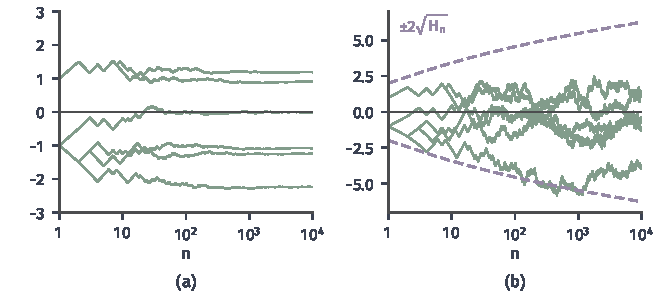
\includegraphics[width=112mm]{figures/07-probability/03-probability-limits/matplotlib/lln-random-harmonic/figure.pdf}
 \caption{同一组随机符号（种子$5$）下两个随机级数的部分和，六条路径，横轴为对数刻度。(a)$\sum_{k\leq n}\varepsilon_k/k$；(b)$\sum_{k\leq n}\varepsilon_k/\sqrt{k}$，紫色虚线为$\pm2\sqrt{H_n}$，$H_n=\sum_{k\leq n}1/k$。}
 \label{fig:lln-random-harmonic}
\end{BookInlineFigure}

\subsection{方差可和的情形}
\label{sec:lln-variance-series}

收敛需要控制部分和的整个尾段，而不仅是某一个时刻的增量。Kolmogorov最大不等式恰好控制一整段路径的最大偏离，把它用在从第$m+1$项开始的尾段上，偏离的概率由尾段方差之和决定。方差可和时，这个尾和趋于零。

\begin{theorem}[方差可和的随机级数]
\label{thm:lln-variance-series}
设$X_1,X_2,\dots$相互独立，$\mathbb{E}[X_k]=0$，并且
\begin{equation}
 \sum_{k=1}^{\infty}\mathbb{E}[X_k^2]<\infty .
 \label{eq:lln-variance-summable}
\end{equation}
则$\sum_kX_k$几乎必然收敛到一个有限的随机变量$S$。此外$S_n\xrightarrow{L^{2}}S$，并且$\mathbb{E}[S]=0$，$\mathbb{E}[S^2]=\sum_k\mathbb{E}[X_k^2]$。
\end{theorem}

\begin{proof}
记$\sigma_k^2=\mathbb{E}[X_k^2]$。对$m\geq0$，令
\[
 V_m=\sup_{j,k>m}\lvert S_j-S_k\rvert,\qquad W_m=\sup_{k>m}\lvert S_k-S_m\rvert ,
\]
二者取值于$[0,\infty]$。$V_m$随$m$不增，所以极限$V=\lim_mV_m$存在，并且部分和是Cauchy列当且仅当$V=0$。对$j,k>m$用三角不等式，
\[
 \lvert S_j-S_k\rvert\leq\lvert S_j-S_m\rvert+\lvert S_k-S_m\rvert\leq2W_m ,
\]
所以$V_m\leq2W_m$。

先估计$W_m$。固定$m$与$\varepsilon>0$，对$N>m$考虑事件
\[
 E_N=\Bigl\{\max_{m<k\leq N}\lvert S_k-S_m\rvert>\varepsilon\Bigr\} .
\]
$E_N$随$N$增大而增大，并上升到$\{W_m>\varepsilon\}$。尾段$S_k-S_m=X_{m+1}+\dots+X_k$是独立中心化变量的部分和，对它用定理~\ref{thm:lln-kolmogorov-maximal}，得到
\[
 \mathbb{P}(E_N)\leq\frac{1}{\varepsilon^2}\sum_{k=m+1}^{N}\sigma_k^2\leq\frac{1}{\varepsilon^2}\sum_{k>m}\sigma_k^2 .
\]
令$N\to\infty$，由概率的连续性，
\begin{equation}
 \mathbb{P}(W_m>\varepsilon)\leq\frac{1}{\varepsilon^2}\sum_{k>m}\sigma_k^2 .
 \label{eq:lln-tail-oscillation}
\end{equation}

再回到$V$。由于$V\leq V_m\leq2W_m$，对每个$m$，
\[
 \mathbb{P}(V>2\varepsilon)\leq\mathbb{P}(W_m>\varepsilon)\leq\frac{1}{\varepsilon^2}\sum_{k>m}\sigma_k^2 .
\]
左边与$m$无关，右边是收敛级数~\eqref{eq:lln-variance-summable}的尾和，令$m\to\infty$趋于零。所以对每个$\varepsilon>0$都有$\mathbb{P}(V>2\varepsilon)=0$。取$\varepsilon=1/j$并对$j$取可数并，得到$\mathbb{P}(V>0)=0$。于是几乎必然地，$S_n$是Cauchy列，收敛到有限极限$S$。

最后看$L^2$收敛。由式~\eqref{eq:lln-sum-variance}，$N>m$时
\[
 \mathbb{E}\bigl[(S_N-S_m)^2\bigr]=\sum_{k=m+1}^{N}\sigma_k^2\leq\sum_{k>m}\sigma_k^2\to0 .
\]
所以$S_n$在$L^2$中是Cauchy列，收敛到某个$S'\in L^2$。由第~\ref{chap:random-variable-convergence}章，$L^2$收敛的序列有几乎必然收敛的子列，其极限只能是$S$，故$S'=S$几乎必然成立。$L^2$收敛蕴含一阶矩与二阶矩收敛，于是
\[
 \mathbb{E}[S]=\lim_{n\to\infty}\mathbb{E}[S_n]=0,\qquad \mathbb{E}[S^2]=\lim_{n\to\infty}\mathbb{E}[S_n^2]=\sum_k\sigma_k^2 .
\]
\end{proof}

证明的结构值得记住：几乎必然收敛归结为“尾段的最大振荡依概率趋于零”，而最大振荡正是Kolmogorov不等式所控制的量。只控制单个增量$S_N-S_m$的方差，只能得到$L^2$收敛，不足以说明每条路径都停下来。

\paragraph{随机调和级数}
对$X_k=\varepsilon_k/k$，各项均值为零，方差可和：
\[
 \mathbb{E}[X_k]=0,\qquad \sum_{k=1}^{\infty}\mathbb{E}[X_k^2]=\sum_{k=1}^{\infty}\frac{1}{k^2}=\frac{\pi^2}{6} .
\]
定理~\ref{thm:lln-variance-series}给出$\sum_k\varepsilon_k/k$几乎必然收敛，极限$S$的均值为$0$，方差为$\pi^2/6\approx1.645$。尾和满足$\sum_{k>m}1/k^2<1/m$，取$\varepsilon=1/4$与$m=100$，式~\eqref{eq:lln-tail-oscillation}给出
\[
 \mathbb{P}\Bigl(\sup_{k>100}\lvert S_k-S_{100}\rvert>\tfrac14\Bigr)\leq16\sum_{k>100}\frac{1}{k^2}\approx16\times0.00995\approx0.159 .
\]

图~\ref{fig:lln-harmonic-limit}(b)把这个界与模拟频率放在一起比较（$4000$条路径，种子$8$，上确界在$k\leq20000$内计算）。$m=100$时模拟频率约为$0.028$。两条曲线都随$m$按$1/m$的阶下降，界比真实值宽松，但单凭方差就保证了尾段的振荡越来越罕见。

\begin{BookInlineFigure}
 \centering
 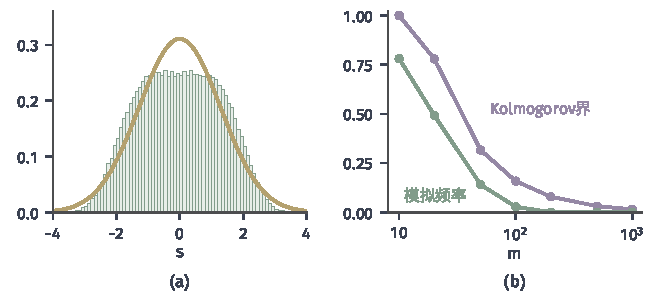
\includegraphics[width=112mm]{figures/07-probability/03-probability-limits/matplotlib/lln-harmonic-limit/figure.pdf}
 \caption{随机调和级数$\sum_k\varepsilon_k/k$的极限与尾段振荡。(a)$S_{1000}$的直方图（浅绿，$200000$个样本，种子$2$）与方差相同的高斯密度$\mathcal{N}(0,\pi^2/6)$（黄线）；(b)尾段最大振荡$\max_{m<k\leq20000}\lvert S_k-S_m\rvert\geq1/4$的模拟频率（绿线，$4000$条路径，种子$8$）与Kolmogorov界$16\sum_{m<k\leq20000}1/k^2$（紫线），横轴为$m$的对数刻度。}
 \label{fig:lln-harmonic-limit}
\end{BookInlineFigure}

极限$S$是一个真正的随机变量，它的分布由全部项共同决定。图~\ref{fig:lln-harmonic-limit}(a)用$S_{1000}$代替$S$，二者之差的方差$\sum_{k>1000}1/k^2$小于$10^{-3}$。直方图顶部平坦，与同方差的高斯密度明显不同。用独立性展开四次方可以核对这一点：对$S_n=\sum_{k\leq n}a_k\varepsilon_k$，奇次项的期望为零，只剩每个下标出现偶数次的项，
\[
 \mathbb{E}[S_n^4]=\sum_{k}a_k^4+3\sum_{j\neq k}a_j^2a_k^2=3\Bigl(\sum_ka_k^2\Bigr)^2-2\sum_ka_k^4 .
\]
取$a_k=1/k$并令$n\to\infty$，用$\sum_k1/k^4=\pi^4/90$，得到
\[
 \frac{\mathbb{E}[S^4]}{(\mathbb{E}[S^2])^2}-3=-\frac{2\pi^4/90}{(\pi^2/6)^2}=-0.8 ,
\]
而高斯分布的这个值为$0$。模拟值约为$-0.81$。

\paragraph{中心化不可省略}
定理要求各项均值为零。若$X_k=1/k$是确定的常数，方差全为零，条件~\eqref{eq:lln-variance-summable}成立，级数却发散。一般地，若$\sum_k\operatorname{Var}(X_k)<\infty$，对$X_k-\mu_k$用定理~\ref{thm:lln-variance-series}，得到$\sum_k(X_k-\mu_k)$几乎必然收敛。两个级数之差是数项级数$\sum_k\mu_k$，所以
\[
 \sum_kX_k\ \text{几乎必然收敛}\iff\sum_k\mu_k\ \text{收敛} ,
\]
并且$\sum_k\mu_k$发散时$\sum_kX_k$几乎必然发散。例如取$X_k=\xi_k/k$，$\xi_k\sim\operatorname{Bern}(1/2)$独立，方差$1/(4k^2)$可和，但均值$1/(2k)$的级数发散，于是$\sum_kX_k=+\infty$几乎必然成立。方差控制随机波动，均值控制系统漂移，两件事要分别检查。

\subsection{截断与大项控制}
\label{sec:lln-truncation}

方差可和是充分条件，但不是必要条件。各项可能偶尔取极大的值，使方差甚至均值都很大或无穷，而这些大值只出现有限次，对级数是否收敛没有影响。

\paragraph{一个方差与均值都失效的例子}
令$X_1=\varepsilon_1$。对$k\geq2$，取与$\varepsilon_k$独立的事件$B_k$，$\mathbb{P}(B_k)=1/k^2$，各$B_k$与各$\varepsilon_k$全体相互独立，定义
\[
 X_k=\begin{cases}k, & B_k\ \text{发生},\\ \varepsilon_k/k, & B_k\ \text{不发生}.\end{cases}
\]
大值$k$出现的机会很小，但幅度很大。逐项计算，$k\geq2$时
\[
 \mathbb{E}[X_k]=k\cdot\frac{1}{k^2}=\frac1k,\qquad
 \operatorname{Var}(X_k)=1+\frac{1}{k^2}-\frac{1}{k^4}-\frac{1}{k^2}=1-\frac{1}{k^4} .
\]
这里用了$\mathbb{E}[X_k^2]=k^2/k^2+(1-1/k^2)/k^2$。方差之和与均值之和都发散，上一小节的判据完全用不上。

然而大项出现的概率可和：
\[
 \sum_{k\geq2}\mathbb{P}(B_k)=\frac{\pi^2}{6}-1\approx0.645<\infty .
\]
由第~\ref{chap:random-variable-convergence}章的Borel–Cantelli引理，几乎必然只有有限个$B_k$发生。对这样的样本点，从某一项起$X_k=\varepsilon_k/k$，而$\sum_k\varepsilon_k/k$几乎必然收敛，改动有限项不影响收敛。所以$\sum_kX_k$几乎必然收敛。

图~\ref{fig:lln-big-terms}画出六条路径（种子$4$）。其中三条各出现一次大项（红点，分别在$k=2,10,2$处），路径随之跳起，此后与其余路径一样停住。黄色虚线是各项期望的累计$\sum_{k\leq n}\mathbb{E}[X_k]$，按$\ln n$无限增长：期望被极少发生的大值撑大，它描述的不是典型路径。

\begin{BookInlineFigure}
 \centering
 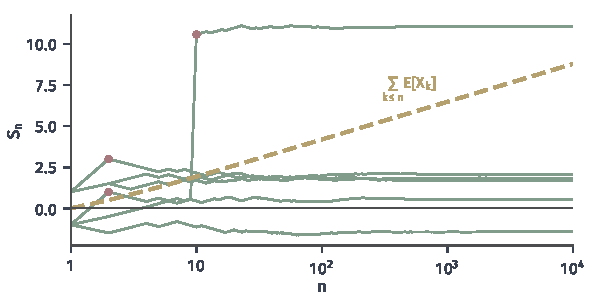
\includegraphics[width=100mm]{figures/07-probability/03-probability-limits/matplotlib/lln-big-terms/figure.pdf}
 \caption{含罕见大项的随机级数，六条路径（种子$4$），横轴为对数刻度。绿线为部分和$S_n$，红点标出大项$X_k=k$出现的位置；黄色虚线为期望的累计$\sum_{k\leq n}\mathbb{E}[X_k]=\sum_{2\leq k\leq n}1/k$。}
 \label{fig:lln-big-terms}
\end{BookInlineFigure}

\paragraph{一般的截断}
这个例子的做法可以一般化：先把大值切掉，再对剩下的有界部分分别处理均值与波动。固定$c>0$，令
\begin{equation}
 Y_k=X_k\mathbf{1}_{\{\lvert X_k\rvert\leq c\}} .
 \label{eq:lln-truncation}
\end{equation}
称$Y_k$为$X_k$在水平$c$处的\term{截断}（truncation）。每一项因此拆成三部分：
\[
 X_k=\bigl(X_k-Y_k\bigr)+\mathbb{E}[Y_k]+\bigl(Y_k-\mathbb{E}[Y_k]\bigr) .
\]
第一部分只在$\lvert X_k\rvert>c$时非零，是大项；第二部分是截断后的均值，一个普通的数；第三部分是有界的中心化波动。

三部分各需要一种控制，图~\ref{fig:lln-truncation-split}画出这种分工。

\begin{BookInlineFigure}
 \centering
 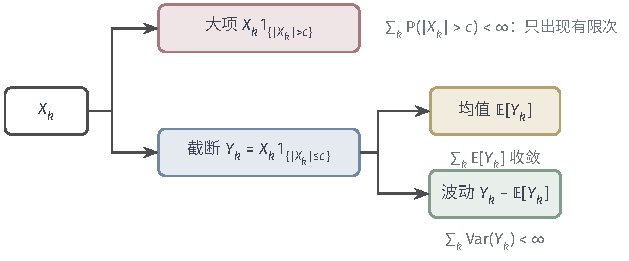
\includegraphics[width=106mm]{figures/07-probability/03-probability-limits/tikz/lln-truncation-split/figure.pdf}
 \caption{在固定水平$c$截断后的三部分及各自的控制条件。浅红框为大项，由超阈值概率之和控制；浅黄框为截断均值，由数项级数控制；浅绿框为中心化波动，由截断方差之和控制。}
 \label{fig:lln-truncation-split}
\end{BookInlineFigure}

\begin{enumerate}
 \item \emph{大项只出现有限次。}若$\sum_k\mathbb{P}(\lvert X_k\rvert>c)<\infty$，由Borel–Cantelli引理，几乎必然存在$N(\omega)$，使$k>N(\omega)$时$X_k(\omega)=Y_k(\omega)$。于是$n>N(\omega)$时$S_n(\omega)-\sum_{k\leq n}Y_k(\omega)$是一个不再变化的有限数，$\sum_kX_k$与$\sum_kY_k$同时收敛或同时发散。这一步不需要独立性，也不要求$X_k$有任何矩。
 \item \emph{截断均值的级数收敛。}$\lvert Y_k\rvert\leq c$，所以$\mathbb{E}[Y_k]$总存在。$\sum_k\mathbb{E}[Y_k]$是一个数项级数，它收敛与否与随机性无关，只能直接检查。
 \item \emph{截断波动的方差可和。}$Y_k-\mathbb{E}[Y_k]$是独立变量$X_k$的函数，彼此独立，均值为零，绝对值不超过$2c$。若$\sum_k\operatorname{Var}(Y_k)<\infty$，由定理~\ref{thm:lln-variance-series}，$\sum_k(Y_k-\mathbb{E}[Y_k])$几乎必然收敛。
\end{enumerate}

三种控制各管一件事。第一种处理方差无法描述的重尾大值；第二种处理系统性漂移；第三种处理有界的随机波动。截断水平$c$固定不变，有界性使第三步可以只用方差。回到上面的例子，取$c=1$：$k\geq2$时$\lvert X_k\rvert>1$恰好是$B_k$发生，$Y_k=\varepsilon_k\mathbf{1}_{B_k^{\mathrm{c}}}/k$，均值为$0$，方差$(1-1/k^2)/k^2$可和，三项都满足。

\subsection{三系列定理}
\label{sec:lln-three-series}

把上一小节的三种控制合在一起，就得到一个随机级数几乎必然收敛的充分条件。Kolmogorov证明了这三个条件也是必要的。

\begin{theorem}[三系列定理]
\label{thm:lln-three-series}
设$X_1,X_2,\dots$相互独立，$c>0$，$Y_k=X_k\mathbf{1}_{\{\lvert X_k\rvert\leq c\}}$。则$\sum_kX_k$几乎必然收敛，当且仅当下面三个级数都收敛：
\begin{equation}
 \sum_{k}\mathbb{P}(\lvert X_k\rvert>c),\qquad
 \sum_{k}\mathbb{E}[Y_k],\qquad
 \sum_{k}\operatorname{Var}(Y_k) .
 \label{eq:lln-three-series}
\end{equation}
\end{theorem}

这一结论称为\term{三系列定理}（three-series theorem）。注意第二个级数只要求收敛，不要求绝对收敛。例如确定的$X_k=(-1)^k/k$，取$c=1$时$Y_k=X_k$，第一、三个级数为零，第二个是条件收敛的交错级数，$\sum_kX_k$确实收敛。

\begin{proof}[充分性的证明]
设三个级数都收敛。由第三个级数与定理~\ref{thm:lln-variance-series}，$\sum_k(Y_k-\mathbb{E}[Y_k])$几乎必然收敛；加上收敛的数项级数$\sum_k\mathbb{E}[Y_k]$，$\sum_kY_k$几乎必然收敛。由第一个级数与Borel–Cantelli引理，几乎必然只有有限个$k$使$X_k\neq Y_k$，所以$\sum_kX_k$与$\sum_kY_k$同时收敛。两个几乎必然事件的交仍是几乎必然事件，结论成立。
\end{proof}

必要性中，第一个级数的必要性可以直接证明。若$\sum_kX_k$几乎必然收敛，则$X_k\to0$几乎必然，所以$\lvert X_k\rvert>c$几乎必然只发生有限次。事件$\{\lvert X_k\rvert>c\}$相互独立；如果$\sum_k\mathbb{P}(\lvert X_k\rvert>c)=\infty$，Borel–Cantelli引理的第二部分会给出它们几乎必然发生无穷多次，矛盾。

另两个级数的必要性需要更细的估计，篇幅较长，读者可查阅~\scite{math-kallenberg2021probability}。其机制是：若截断方差之和发散，有界独立波动的累计会像标准差$\sqrt{\sum_{k\leq n}\operatorname{Var}(Y_k)}$那样不断扩大，不可能停在一处，这与图~\ref{fig:lln-random-harmonic}(b)的情形相同；方差可和而均值级数发散时，前面已经说明级数几乎必然发散。同一参考书还说明，独立随机级数收敛的概率只能是$0$或$1$，所以三个级数中只要有一个发散，$\sum_kX_k$就几乎必然发散。

\paragraph{截断水平的选择}
定理对每个固定的$c>0$都成立。由必要性，若三个级数对某个$c$都收敛，则级数收敛，从而它们对所有$c>0$都收敛。实际使用时取最方便的$c$即可。

\paragraph{随机符号级数}
设$(a_k)$是有界实数列，考虑$\sum_ka_k\varepsilon_k$。取$c>\sup_k\lvert a_k\rvert$，截断不改变任何一项：第一个级数为零，$\mathbb{E}[Y_k]=0$，$\operatorname{Var}(Y_k)=a_k^2$。由三系列定理，
\begin{equation}
 \sum_ka_k\varepsilon_k\ \text{几乎必然收敛}\iff\sum_ka_k^2<\infty .
 \label{eq:lln-random-signs}
\end{equation}
取$a_k=k^{-p}$，随机符号的$p$级数几乎必然收敛当且仅当$p>1/2$。这是“抵消到什么程度”的确切答案：确定的$p$级数需要$p>1$，随机符号使门槛降到$p>1/2$，因为抵消后累计量按平方和的平方根增长。$p=1/2$正是图~\ref{fig:lln-random-harmonic}(b)的情形，那里的发散用到了这里引用的必要性部分。

后面的强大数律只用到方差可和的情形，即定理~\ref{thm:lln-variance-series}。三系列定理的作用是说明这个工具在独立级数问题中已经足够：截断之后，收敛与否就由方差和均值决定。
